\section{Datasets and experimental results analysis}
\label{sec:results}

\subsection{Datasets}
Table~\ref{tab:data} lists the data. The public room is \texttt{vr\_room} from MuSHRoom \cite{ren2024mushroom} (CC BY 4.0), a room with plain concrete walls, chosen because it has the same kind of data as our phones (iPhone images, ARKit poses, LiDAR depth) plus a laser-scanned reference mesh. Its long capture trains the model with every tenth frame held out (the ``within'' test); its separate short capture, from viewpoints the training walk did not take, is the harder ``with'' test. Our own room is a bedroom captured three times by Sejal Satheesh on an iPhone~13~Pro; every eighth frame of the used capture is held out.

\begin{table}[!htb]
\caption{Datasets. Held-out frames are never used for training.}
\label{tab:data}
\centering
\small
\begin{tabular}{L{3.4cm}L{3.2cm}L{2.5cm}L{3.3cm}}
\hline
\textbf{Room / sequence} & \textbf{Source, device} & \textbf{Frames} & \textbf{Used for} \\
\hline
\texttt{vr\_room} long capture & MuSHRoom, iPhone & 422 (42 held out) & training, ``within'' test \\
\texttt{vr\_room} short capture & MuSHRoom, iPhone & 186 & ``with'' test \\
\texttt{vr\_room} laser scan & MuSHRoom reference & -- & mesh and collision reference \\
Own room \texttt{cap1} & iPhone 13 Pro, Polycam & 32 & capture check (too sparse) \\
Own room \texttt{cap2} & iPhone 13 Pro, Polycam & 257 (33 held out) & training, walk, capture check \\
Own room \texttt{cap3} & iPhone 13 Pro, Polycam & 491 (3 segments) & capture check, tracking repair \\
ARKitScenes 41254269 & iPad Pro & 95\,s walk & v1 only \\
\hline
\end{tabular}
\end{table}

\textbf{Experimental setup.} Training, export and mesh evaluation ran on a shared GPU machine: an NVIDIA A100-PCIE-40GB (MIG 7g.40gb) of which another user held 33--35\,GB, with 96 CPU cores and 188\,GB RAM, in an Ubuntu 20.04 container. The environment was built with pixi \cite{pixi}: Python 3.10, PyTorch 2.2.2 with CUDA 11.8, nerfstudio 1.1.3, gsplat 1.0.0 and DN-Splatter at commit 97588b4 \cite{dnsplattercode}. Each room was trained for 30,000 steps (Table~\ref{tab:settings}) and evaluated on all held-out images every 1,000 steps. Mesh accuracy follows DN-Splatter's MuSHRoom protocol: the mesh is aligned to the scan with the dataset's ICP transform, both are culled to what the capture saw, and accuracy (mesh to scan), completeness (scan to mesh) and F-score at 5\,cm are reported. ``Plain splats'' is the same model with every prior switched off and 3D instead of flattened Gaussians, trained with the same data and settings. Collision, walking and the collision evaluation ran on the laptop (Windows~11, RTX~3050 Laptop GPU with 6\,GB, Chrome, SuperSplat Viewer 1.37.0, splat-transform 3.9.0--3.10.1, Python with NumPy and SciPy).

\subsection{Reconstruction quality}
On \texttt{vr\_room} (Table~\ref{tab:quality}), DN-Splatter's priors cost 0.5\,dB of PSNR on held-out frames of the training walk but gain 0.26\,dB on the separate walk, and its mesh is 3.3 times closer to the laser scan (1.76 vs 5.85\,cm, F-score 0.93 vs 0.64). Since walk collision is built from geometry, we kept DN-Splatter. Neither run collapsed (Figure~\ref{fig:curves}, right). Our own room reached 22.2\,dB on its held-out frames, a different room and capturer, so not directly comparable. Training took 87 minutes (DN-Splatter) and 79 minutes (plain) on \texttt{vr\_room}, and 99 minutes on our room including one crash and automatic resume; our peak GPU memory was about 5.2--5.3\,GB, and the final splats held 0.91\,M and 0.75\,M Gaussians.

\begin{table}[!htb]
\caption{Reconstruction quality after 30,000 steps (GPU machine). Depth is compared with the phone's LiDAR, on which DN-Splatter trains, so that column favours it; mesh metrics are against the laser scan.}
\label{tab:quality}
\centering
\begin{adjustbox}{max width=\linewidth}
\begin{tabular}{lccccccccc}
\hline
\multirow{2}{*}{\textbf{Run}} & \multicolumn{3}{c}{\textbf{Within}} & \multicolumn{3}{c}{\textbf{With}} & \textbf{Depth} & \textbf{Mesh acc.} & \textbf{F-score} \\
 & PSNR & SSIM & LPIPS & PSNR & SSIM & LPIPS & abs.\ rel. & (cm) & @5\,cm \\
\hline
\texttt{vr\_room}, plain splats & \textbf{26.84} & \textbf{0.875} & \textbf{0.124} & 23.24 & \textbf{0.818} & 0.192 & 0.056 & 5.85 & 0.638 \\
\texttt{vr\_room}, DN-Splatter & 26.32 & 0.862 & 0.143 & \textbf{23.50} & 0.812 & 0.192 & \textbf{0.016} & \textbf{1.76} & \textbf{0.926} \\
Own room, DN-Splatter & 22.18 & 0.853 & 0.170 & -- & -- & -- & 0.017 & -- & -- \\
\hline
\end{tabular}
\end{adjustbox}
\end{table}

Figure~\ref{fig:renders} shows renders next to the photographs. Near the training walk, signs, pipes and the door are sharp; from the other walk, the blanket and the wall seen close up are streaky. In our room the patterned mattress is sharp but the plain walls and ceiling are smeared. Plain walls remain the weak point even with depth and normal priors.

\begin{figure}[!htb]
	\centering
	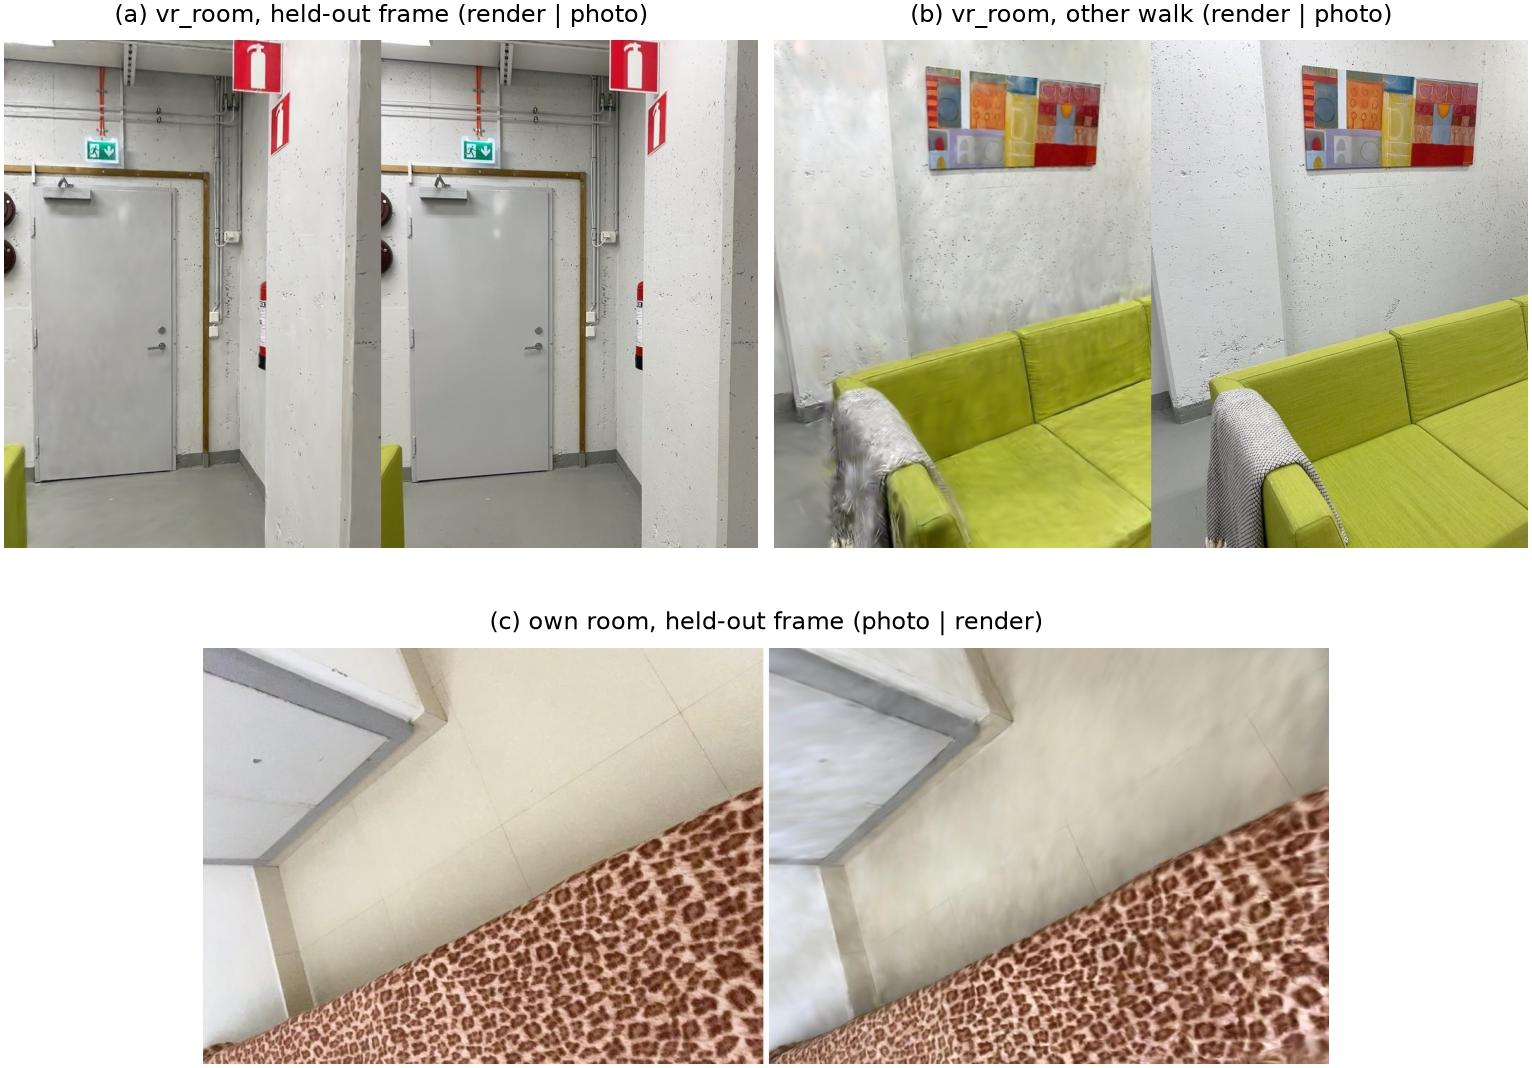
\includegraphics[width=0.9\linewidth]{figures/renders.jpg}
	\caption{Renders on held-out frames (GPU machine). (a) A held-out frame of the \texttt{vr\_room} training walk and (b) a frame of its separate walk, render left; (c) our own room, render right.}
	\label{fig:renders}
\end{figure}

\subsection{Walkability}
Both rooms were walked in the SuperSplat Viewer on the laptop (Table~\ref{tab:walk}). In \texttt{vr\_room} the walker starts inside the room at eye height, walls stop the walker at the visible surface and the floor holds; our own room was judged good by Aswin, without recording each check. In both screen recordings the overlay showed a frame time of 10.0\,ms at every sampled moment while the GPU time varied, which suggests the display, not rendering, set the frame rate. Close to a million Gaussians therefore needed no pruning, unlike the 400--500k limit of v1's browser viewer.

\begin{table}[!htb]
\caption{Walk tests (laptop, Chrome). Times are read from the viewer's overlay in the screen recordings at regular samples.}
\label{tab:walk}
\centering
\small
\begin{tabular}{lccccc}
\hline
\textbf{Room} & \textbf{Gaussians} & \textbf{Spawn inside} & \textbf{Walls stop, floor holds} & \textbf{Frame} & \textbf{GPU} \\
\hline
\texttt{vr\_room} & 908k & yes & yes & 10.0\,ms & 2.5--8.3\,ms \\
Own room & 746k & \multicolumn{2}{c}{judged good (not itemised)} & 10.0\,ms & 2.9--7.1\,ms \\
\hline
\end{tabular}
\end{table}

\subsection{Walk-collision accuracy}
\label{sec:collision-results}
Table~\ref{tab:collision} and Figure~\ref{fig:collision} give the collision study. The default collision from the splat (S) has gaps at body height, along one wall and at furniture, so the walkable area leaks out of the room (11.3\,m$^2$ against the scan's 6.5\,m$^2$): IoU 0.58, with 17.8\% of the walls the phone saw missing. Collision from DN-Splatter's mesh (M) follows the scan closely: IoU 0.81, 1.7\% missed, and a 95th-percentile offset of 10 instead of 20\,cm, but with 0.04\,m$^2$ of phantom obstacles (16 cells of 5\,cm) where S has none. M therefore passes P1, P3 and P4 (the median offset ties at 0 at this resolution) and fails P2, so the all-four rule we set is not met. Raw phone LiDAR (L) is unusable for collision (IoU 0.06, 4.3\,m$^2$ of phantom obstacles from noise and stray points), so the training step that filters the depth matters. Polycam's mesh (P), aligned in its best case, is almost as good as M but with more phantom obstacles.

\begin{table}[!htb]
\caption{Walk-collision accuracy against the laser scan of \texttt{vr\_room} (laptop). All sources use the same splat-transform pipeline; measured on a 5\,cm grid between 0.2 and 1.8\,m above the floor.}
\label{tab:collision}
\centering
\small
\begin{tabular}{lccccc}
\hline
\textbf{Source} & \textbf{IoU $\uparrow$} & \textbf{Phantom $\downarrow$} & \textbf{Missed $\downarrow$} & \textbf{Offset med./p95} & \textbf{Walkable} \\
\hline
S: splat (default) & 0.577 & \textbf{0.00}\,m$^2$ & 17.8\% & 0 / 20\,cm & 11.3\,m$^2$ \\
M: DN-Splatter mesh & \textbf{0.809} & 0.04\,m$^2$ & \textbf{1.7\%} & 0 / \textbf{10}\,cm & 7.6\,m$^2$ \\
P: Polycam mesh & 0.794 & 0.22\,m$^2$ & 1.8\% & 0 / 10\,cm & 6.9\,m$^2$ \\
L: raw phone LiDAR & 0.059 & 4.27\,m$^2$ & 47.0\% & 5 / 41\,cm & 11.4\,m$^2$ \\
GT: laser scan & 1 & 0 & 0\% & 0 / 0\,cm & 6.5\,m$^2$ \\
\hline
\end{tabular}
\end{table}

\begin{figure}[!htb]
	\centering
	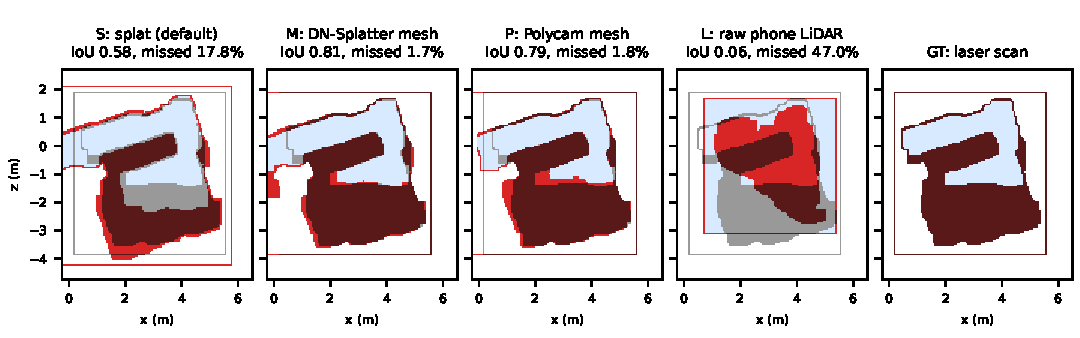
\includegraphics[width=\linewidth]{figures/collision.pdf}
	\caption{Floor plans of the \texttt{vr\_room} walk collision at body height. Red: the source's collision; grey: the laser scan's; dark red: both; light blue: walkable from the spawn. The outer rectangles close each collision volume's bounding box.}
	\label{fig:collision}
\end{figure}

The difference was not felt in practice: walking both versions freely, Aswin noticed no difference between S and M. The gaps lie at furniture and wall stretches that a free walk did not reach. The study has clear limits: one room (the only one of ours with a laser scan); the reference is the scan's own collision through the same 5\,cm pipeline; the 5\,cm cells make the median offset coarse; and S uses the real Gaussians while M, L, P and GT were converted into 2\,cm splats, which may itself contribute to the difference.

\subsection{Negative results: capture check and tracking repair}
\label{sec:negative}
\label{sec:capcheck}
\textbf{Capture check.} Its verdicts matched what we knew: \texttt{cap3} was flagged as broken tracking (Figure~\ref{fig:capcheck}, left), and \texttt{cap1}, \texttt{cap2} and \texttt{vr\_room} were asked to recapture some areas but not flagged as broken; it ran in 18--52\,s per room on the laptop. Its pre-agreed validation, comparing labels with the trained model's error on held-out frames, failed both criteria (Table~\ref{tab:capcheck}). Under-covered patches had only slightly higher error than OK patches, with overlapping intervals, and textureless patches had \emph{lower} error. Coverage predicted the worst 20\% of patches no better than chance (AUC 0.53--0.54), and texture added 0.046 AUC, short of the 0.05 required. A likely reason, found afterwards, is that a per-pixel colour error rewards smooth renders of plain walls: with 1$-$SSIM as the error (not pre-agreed), texture separated bad patches with an AUC of 0.73--0.82, in the direction ``more detail, more error''. The check is kept as a fallback, not claimed as a result.

\begin{table}[!htb]
\caption{Capture-check validation (laptop): mean held-out patch error (absolute colour error, 0--1) with bootstrap 95\% intervals. The criterion required under-covered and textureless patches to exceed OK patches with non-overlapping intervals in the test room.}
\label{tab:capcheck}
\centering
\small
\begin{tabular}{lccc}
\hline
\textbf{Room} & \textbf{OK} & \textbf{Under-covered} & \textbf{Textureless} \\
\hline
\texttt{vr\_room} (calibration) & 0.033 [0.029, 0.036] & 0.036 [0.033, 0.039] & 0.016 [0.010, 0.022] \\
\texttt{cap2} (test) & 0.056 [0.049, 0.065] & 0.063 [0.053, 0.074] & 0.034 [0.020, 0.057] \\
\hline
\end{tabular}
\end{table}

\begin{figure}[!htb]
	\centering
	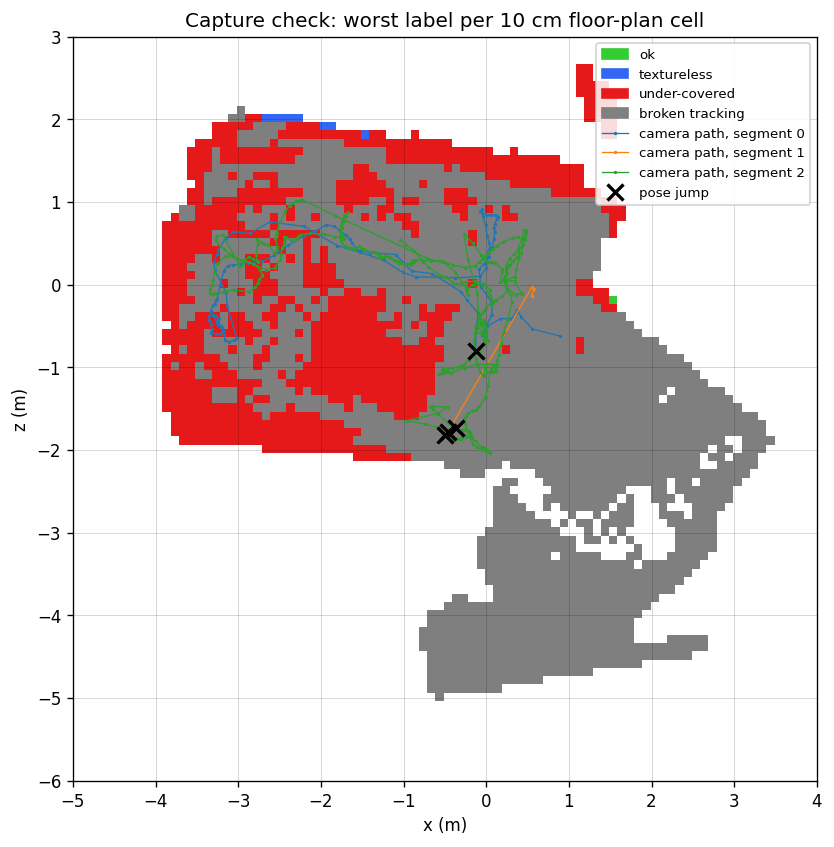
\includegraphics[height=5.6cm]{figures/capcheck_cap3.png}\hfill
	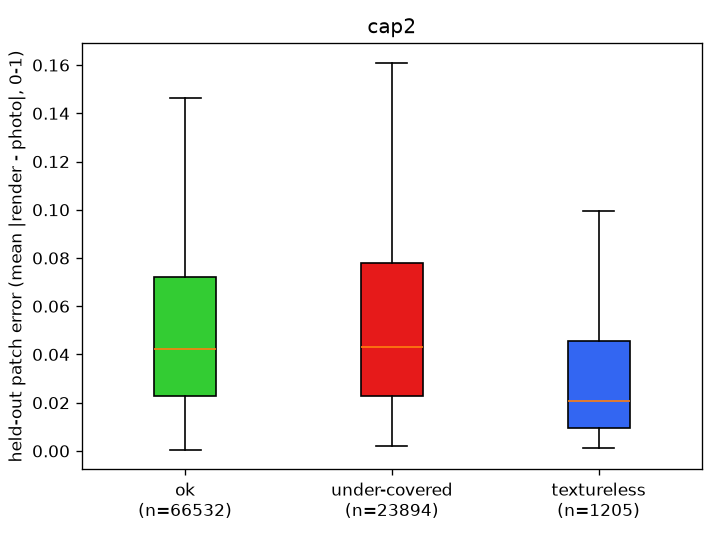
\includegraphics[height=5.6cm]{figures/capcheck_error_cap2.png}
	\caption{Capture check. Left: top-down map of \texttt{cap3}, worst label per 10\,cm cell, with the camera path coloured by tracking segment and pose jumps marked; grey areas were seen only by frames with broken tracking. Right: held-out patch error by label in the test room; textureless patches have lower error, against the check's claim.}
	\label{fig:capcheck}
\end{figure}

\textbf{Tracking repair.} The second attempt registered \texttt{cap3}'s separate sweeps to each other before training. The registration worked (fitness 0.87, turn $-0.9^\circ$, tilt $0.6^\circ$), but there was nothing to repair: before any repair the first sweep's depth already lay within 2.4\,cm of the main sweep with Polycam's corrected poses (2.7\,cm with ARKit's), close to the main sweep's 1.9\,cm agreement with itself. ARKit had relocalised, and only seven transition frames (118--124) carried the 2\,m jumps. The pre-agreed premise was false, and the added surface (4.7\%) fell below the required 5\%.

\subsection{Comparison with existing implementations}
Table~\ref{tab:compare} compares existing ways to obtain the model or its walk collision with our pipeline, all run and measured by us on \texttt{vr\_room}. Plain splats render the training walk best but give the least accurate geometry; the viewer's default collision from the splat leaks out of the room; raw phone LiDAR cannot be used for collision; and Polycam's mesh gives collision almost as good as ours, with more phantom obstacles (we did not evaluate the app's other outputs). Our combination, DN-Splatter's splat for viewing and its mesh for collision, has the most accurate geometry and the best collision on every measure except phantom obstacles.

\begin{table}[!htb]
\caption{Comparison of existing implementations with ours on \texttt{vr\_room} (our measurements; ``--'': not applicable or not measured).}
\label{tab:compare}
\centering
\begin{adjustbox}{max width=\linewidth}
\begin{tabular}{L{5.2cm}cccccc}
\hline
\textbf{Method (implementation)} & \textbf{PSNR within / with} & \textbf{Mesh acc.} & \textbf{F@5\,cm} & \textbf{Walk IoU} & \textbf{Phantom} & \textbf{Missed} \\
\hline
Plain 3DGS splats \cite{kerbl3dgs} (nerfstudio, priors off) & \textbf{26.84} / 23.24\,dB & 5.85\,cm & 0.638 & -- & -- & -- \\
SuperSplat default: collision from the splat \cite{splattransform} & same splat as ours & -- & -- & 0.577 & \textbf{0.00}\,m$^2$ & 17.8\% \\
Raw phone LiDAR, no reconstruction & -- & -- & -- & 0.059 & 4.27\,m$^2$ & 47.0\% \\
Polycam app mesh \cite{polycam} & -- & -- & -- & 0.794 & 0.22\,m$^2$ & 1.8\% \\
\textbf{Ours}: DN-Splatter splat + mesh collision & 26.32 / \textbf{23.50}\,dB & \textbf{1.76\,cm} & \textbf{0.926} & \textbf{0.809} & 0.04\,m$^2$ & \textbf{1.7\%} \\
\hline
\end{tabular}
\end{adjustbox}
\end{table}
